%%
%% Author: thompson
%% 25.11.17
%%

% Preamble
\documentclass[11pt]{article}

% Packages
\usepackage{a4wide}
\usepackage[ngerman]{babel}
\usepackage[utf8]{inputenc}

\usepackage{scrextend}
\usepackage{enumerate}
\usepackage{graphicx}
\usepackage{listings}


% Document
\begin{document}
    \lstset{language=C++}
    \graphicspath{{PictureDoc/}}


    \section{OMNeT++}
    \subsection{Q\&A}

    \begin{enumerate}[\thesubsection .1]
        \item Wie wird eine Topologie erstellt und dessen Funktionalität realisiert?\\\\
        Eine Topologie, sprich eine Simulation wird in OMNeT++ mithilfe mehrerer Datentypen definiert. Es gibt:
        \begin{enumerate}[$\circ$]
            \item .NED - \textbf{NE}twork \textbf{D}escription File
            In diesen beschreibt man, wie der Name bereits verät, das Netzwerk mit all dessen Knoten, Empfängern wie Sendern.
            Neben den DataNodes beschreibt man auch den groben Funktionsumfang, etwa wann Daten gesendet werden sowie Delay.
            Mithilfe 2er Modi: Source und Design lässt sich das Netzwerk graphisch als auch programmiertechnisch beliebig anpassen.\\

            \item .CC - C++ Datensätze:\\
            In diesen beschreibt man die Subfunktionen e.g. das Verhalten aller Instanzen innerhalb des Netzwerkes.
            Für gewöhnlich bedient man sich vordefinierten Spezifikationen wie cMessage oder cSimpleModule, von welchen
            die eigenen Klassen erben.\\
            \item .INI - Initialisierungsdatei
            Diese beschreibt das zu simulierende Netzwerk, definiert im .NED-File.
            \emph{Es gilt die Klasse anzugeben, nicht den Dateinamen.\\}
        \end{enumerate}

        \item Wie kompiliert und startet eine Simulation?\\
        Prinzipiell mithilfe des RUN-Buttons der IDE.

        Für gewöhnlich gilt es mithilfe von cpp-makemake ein File zu erstellen, welches dann ausgeführt wird.
        Dieses orientiert sich an der jeweiligen omnetpp.ini-Datei, worin die auszuführenden Daten spezifiziert sind.
        Ähnlich einer Kettenreaktion wird dann der Rest ausgelesen, kompiliert und ausgeführt.\\

        \item Wie fügt man folgende hinzu:
        \begin{addmargin}[1em]{1em}
            \begin{enumerate}
                \item{Graphische Elemente:\\\\}
                Werden üblicherweise mithilfe der .ned Datei erstellt.
                Hierbei wird der TicToc mittels des network Blocks als Netzwerk
                gekennzeichnet.\\

                \item{Ausgabe zur Fehlersuche:\\\\}
                Ausgaben werden können über Logger oder über folgenden Befehl ausgegeben werden:
                \begin{lstlisting}
                    EV << "Sending initial message";
                \end{lstlisting}
                \item{Zustandsvariablen:\\\\}
                Werden innerhalb einer Klasse definiert.

                \begin{lstlisting}
                    private:
                    int counter
                \end{lstlisting}

                \item{Zufällige Parameter:\\\\}
                Über Parameter eines Moduls können zufällige Werte generiert werden.
                Um diese letztendlich verwenden zu können, werden sie innerhalb der
                handleMessage() Methode eingelesen.
                Beispiel:\\
                \begin{lstlisting}
                    simtime_t delay = par("delayTime");
                    EV << "Message arrived, starting to wait ";
                    tictocMsg = msg;
                    scheduleAt(simTime()+delay, event);
                \end{lstlisting}
                Die Parameter werden hierbei über die .ini Datei übergeben.

                \begin{lstlisting}
                    Tictoc.tic.delayTime = exponential(3s)
                    Tictoc.toc.delayTime = truncnormal(3s, 1s)
                \end{lstlisting}
            \end{enumerate}

        \end{addmargin}


        \item Wie setzt man Vererbung, Verzögerung, Zeitüberschreitung um oder hebt diese auf?\\


        \begin{enumerate}
            \item Vererbung:\\
            Umsetzung:\\
            Aufhebung:\\

            \item Verzögerung:\\
            Umsetzung:\\
            Verzögerungen können mittels dem Aufruf der Methode scheduleAt() realisiert werden.\\
            Beispiel: scheduleAt(simTime()+1.0, event);\\
            Aufhebung:\\

            \item Zeitüberschreitung:\\
            Umsetzung:\\
            Aufhebung:\\

            \item{}
        \end{enumerate}

        \item Wie funktionieren Netzwerktopologien mit mehr als 2 Knoten?\\
        \begin{enumerate}
            \item{zuerst muss in der .ned-Datei angegeben werden, dass mehrere Input/Output Gates enthalten sind, wobei [ ]
            die eigentliche Gates in Gate Vektoren ändert}
            \begin{lstlisting}
                gates:
                input in[];
                output out[];
            \end{lstlisting}
            \item{im nächsten Schritt werden die Module erstellt und miteinander verbunden\\}
            \item{wurden die Module erstellt und verbunden so kann das Programm gestartet werden\\}
            \item{Funktionsweise einer solche Topologie sieht wie folgt aus:\\}

            Ein Knoten erstellt hierbei die Nachricht, welche letztendlich durch einen
            anderen Knoten im Netzwerk in verschiedenen Richtungen solange weiterverbreitet
            wird bis ein vordefinierter Zielknoten erreicht wird.
        \end{enumerate}

        \item Wie wird ein eigenes Nachrichtenformat definiert und wie werden sie verwendet?\\\\
        Nachrichten können auf zwei Arten erstellt werden:\\
        \begin{enumerate}
            \item{ indem eine eigene Unterklasse von cMessage erstellt, in der ein
            Ziel als Datenelement hinzugefügt wird.\\}
            \item{oder man erstellt eine eigene Message Klasse die wie folgt aussehen könnte:\\\\}
            \begin{lstlisting}
                message TicTocMsg13
                {
                int source;
                int destination;
                int hopCount = 0;
                }
            \end{lstlisting}
        \end{enumerate}

        Verwendet wird die Nachricht dann wie folgt:\\
        \begin{enumerate}
            \item{zuerst muss die erzeugte .msg-Datei mittels
            des message compilers kompiliert werden, wodurch tictoc.h
            und tictoc.cc erzeugt werden (beinahlten die erstellte TicTocMsg Klasse,
            welche Unterklasse von cMessage ist und getter/setter enthalten)\\}

            \item{im nächsten Schritt muss die erzeugte Klasse importiert werden}
            \begin{lstlisting}
                #include "tictoc1
            \end{lstlisting}


            \item{um die Message verwenden zu können, wird sie innerhalb der C++ Datei
            wie folgt erstellt:\\}
            \begin{lstlisting}
                TicTicMsg13 *msg generateMessage(){
                TicTocMsg13 *msg = new TicTocMsg13(msgname);
                msg->setSource(src);
                msg->setDestination(dest);
                return msg;
                }
            \end{lstlisting}

            \item{die handleMessage Methode muss nun wie folgt beginnen:\\}

            \begin{lstlisting}
                void Txc13::handleMessage(cMessage *msg){
                TicTocMsg13 *ttmsg = check_and_cast<TicTocMsg13 *>(msg);
                etc.
                }
            \end{lstlisting}
            Das Argument, welches der handleMessage() übergeben wird, ist die Message,
            die wir als cMessage übergeben bekommen. Hierbei können wir nur dann auf
            dessen Felder zugreifen, wenn wir die Message zu TicTocMsg13* casten.
            Ein einfacher C-Style cast zu einem Crash führen würde, sollte die Message
            eine TicTocMsg13 sein. Daher ermöglicht C++ das verwenden von dynamischen casts,
            wie in unserem Fall:
            \begin{lstlisting}
                check_and_cast<>()
            \end{lstlisting}
            Es versucht hier den Pointer mithilfe eines dynamischen casts umzuwandeln. Sollte
            dieser jedoch fehlschlagen, so wird eine ERROR MESSAGE aufgegeben.

        \end{enumerate}

        \item Statistiken, Auswertung und Visualisierung - Wie setzt man sie um?\\

        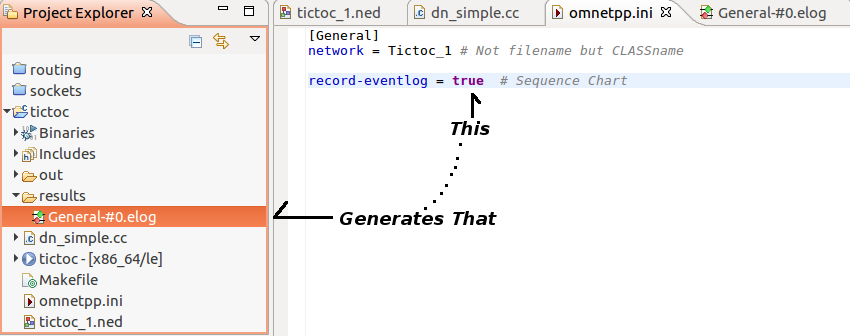
\includegraphics[width=\textwidth]{charting1.png}

        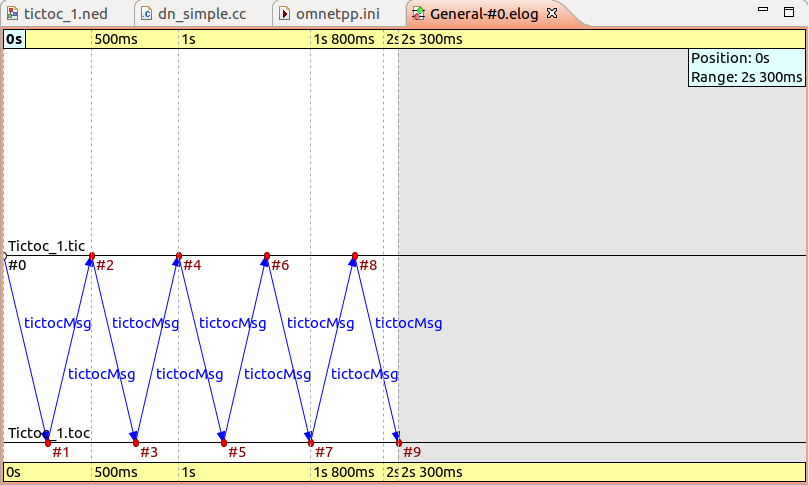
\includegraphics[width=\textwidth]{charting2.png}


    \end{enumerate}
\end{document}